\documentclass[14pt]{extarticle}

\usepackage[T1]{fontenc}
\usepackage[utf8]{inputenc}

\usepackage[hidelinks]{hyperref}

\usepackage{microtype}

\usepackage{amssymb}
\usepackage{amsmath}
\usepackage{mathtools}
\usepackage{dsfont}

\usepackage{enumitem}

\usepackage{tikz}
\usetikzlibrary{cd, patterns, patterns.meta, decorations.pathmorphing}

\usepackage{geometry}
\geometry{a4paper, total={170mm, 252mm}, top=22mm}

\usepackage[skip=7pt]{parskip}

\usepackage{amsthm}
\usepackage{thmtools}

\newtheoremstyle{straightstyle}
  {6pt} % Space above
  {6pt} % Space below
  {} % Body font
  {} % Indent amount
  {\bfseries} % Theorem head font
  {.} % Punctuation after theorem head
  {.5em} % Space after theorem head
  {} % Theorem head spec (can be left empty, meaning `normal')

\newtheoremstyle{italicsstyle}
  {6pt} % Space above
  {6pt} % Space below
  {\slshape} % Body font
  {} % Indent amount
  {\bfseries} % Theorem head font
  {.} % Punctuation after theorem head
  {.5em} % Space after theorem head
  {} % Theorem head spec (can be left empty, meaning `normal')

\declaretheorem[ %
  name=Definition, %
  numberwithin=section, %
  style=italicsstyle
]{definition}

\declaretheorem[ %
  name=Theorem, %
  numberwithin=section, %
  style=straightstyle
]{theorem}

\declaretheorem[ %
  name=Proposition, %
  numberlike=theorem, %
  style=straightstyle
]{proposition}

\declaretheorem[ %
  name=Corollary, %
  numberlike=theorem, %
  style=straightstyle
]{corollary}

\declaretheorem[ %
  name=Lemma, %
  numberlike=theorem, %
  style=straightstyle
]{lemma}

\declaretheorem[ %
  name=Remark, %
  numberlike=definition, %
  style=italicstyle
]{remark}

\declaretheorem[ %
  name=Example, %
  numberwithin=section, %
  style=straightstyle
]{example}


% \renewenvironment{proof}{{\bfseries Proof}$ $\newline}{
%   \begin{flushright} $ \spadesuit $ \end{flushright}$ $\newline
% }

\usepackage{cleveref}

%\crefname{definition}{definicja}{definicje}
%\Crefname{definition}{Definicja}{Definicje}
%
%\crefname{theorem}{twierdzenie}{twierdzenia}
%\Crefname{theorem}{Twierdzenie}{Twierdzenia}
%
%\crefname{lemma}{lemat}{lematy}
%\Crefname{lemma}{Lemat}{Lematy}
%
%\crefname{remark}{uwaga}{uwagi}
%\Crefname{remark}{Uwaga}{Uwagi}


\DeclareMathOperator{\Z}{\mathbb{Z}}
\DeclareMathOperator{\R}{\mathbb{R}}
\DeclareMathOperator{\C}{\mathbb{C}}
\DeclareMathOperator{\N}{\mathbb{N}}
\DeclareMathOperator{\Q}{\mathbb{Q}}

\DeclareMathOperator{\im}{im}
\DeclareMathOperator{\coker}{coker}

\newcommand{\set}[1]{\mathcal{#1}}


\DeclareMathOperator{\ord}{ord}
\DeclareMathOperator{\Ann}{Ann}
\DeclareMathOperator{\Hom}{Hom}

\DeclareMathOperator{\Col}{Col}

\DeclareMathOperator{\End}{End}

\let\landtemp\land
\renewcommand{\land}{\;\landtemp\;}





\usepackage{tikz}
\usetikzlibrary{spath3, hobby, knots, braids}

\pgfdeclarelayer{bg}    % declare background layer
\pgfsetlayers{bg,main}

\title{A voyage into the algebras}
\author{
  Weronika Jakimowicz\\
  330006
  \and 
  Julia Walczuk\\
  332742
}
\date{2023-2024}

\begin{document}
\maketitle
\bigskip

\begin{center}
  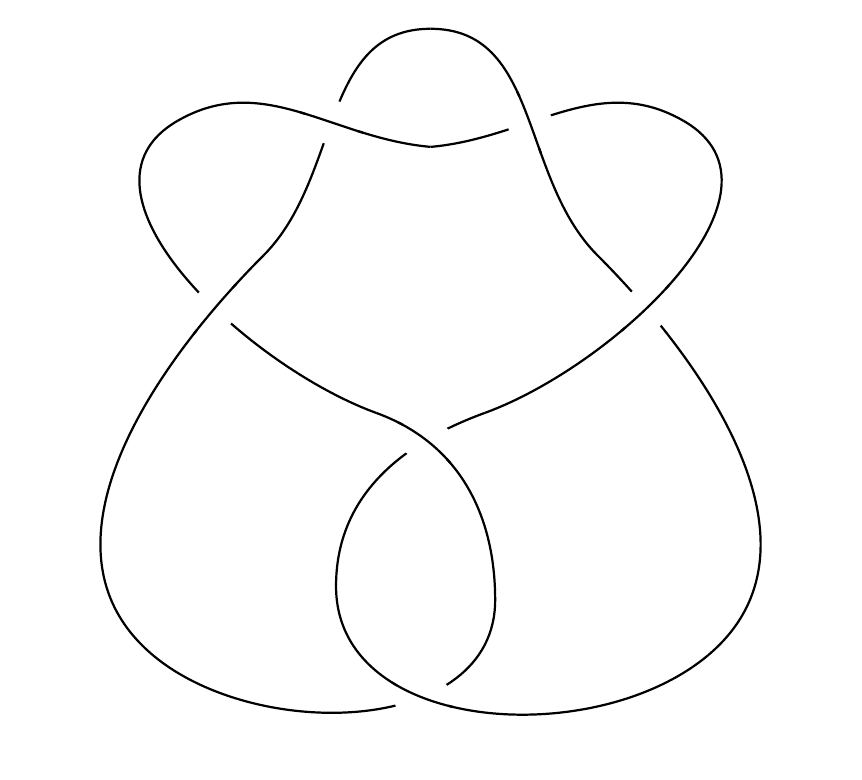
\begin{tikzpicture}[bgnd/.style={circle, fill=white, draw=white}]
    %\node[opacity=0.2] at (0,0) {\includegraphics[width=0.7\textwidth]{./rozdzialy/6_1-3d.png}};

    \coordinate (a0) at (0,0);
    \coordinate (a1) at (90:5);
    \coordinate (a2) at (45:3);
    \coordinate (a3) at (-40:4.6);
    \coordinate (a4) at (-120:2.4);
    \coordinate (a5) at (10:0.7);
    \coordinate (a6) at (50:5);
    \coordinate (a7) at (90:3.5);
    \coordinate (a8) at (180-50:5);
    \coordinate (a9) at (170:0.7);
    \coordinate (a10) at (-70:2.4);
    \coordinate (a11) at (220:4.6);
    \coordinate (a12) at (180-45:3);

    %\foreach \i in {0,...,12} \fill (a\i) circle (2pt);

    \begin{knot}[
      clip width=20, 
      flip crossing=1,
      flip crossing=3,
      flip crossing=6
      ]
      \strand[thick] (a1) to[out=0, in=90+45] (a2) to[out=-45, in=40] (a3);
      \strand[thick] (a3) to[out=220, in=-90] (a4) to[out=90, in=200] (a5);
      \strand[thick] (a5) to[out=20, in=-30] (a6);
      \strand[thick] (a6) to[out=150, in=5] (a7);
      \strand[thick] (a7) to[out=175, in=30] (a8);
      \strand[thick] (a8) to[out=210, in=160] (a9);
      \strand[thick] (a9) to[out=-20, in=90] (a10);
      \strand[thick] (a10) to[out=-90, in=-40] (a11);
      \strand[thick] (a11) to[out=140, in=180+45] (a12);
      \strand[thick] (a12) to[out=45, in=180] (a1);
    \end{knot}

    %\node at (80: 5) {$A$};
    %\node at (-40:4) {$B$};
    %\node at (45:5.5) {$C$};
    %\node at (135:5.5) {$D$};
    %\node at (-1.5,0.1) {$E$};
    %\node at (220:4) {$F$};
    %
    %\node[bgnd] at (70:4.7) {$1$};
    %\node[bgnd] at (25:3.9) {$2$};
    %\node[bgnd] at (-90:3) {$3$};
    %\node[bgnd] at (90:0.5) {$4$};
    %\node[bgnd] at (110:4.7) {$5$};
    %\node[bgnd] at (180-25:3.9) {$6$};

    %\draw[dashed] (70: 4) circle (0.4);
    %\draw[dashed] (28: 3.1) circle (0.4);
    %\draw[dashed] (-90:3.5) circle (0.4);
    %\draw[dashed] (-90:0.15) circle (0.4);
    %\draw[dashed] (180-28:3.1) circle (0.4);
    %\draw[dashed] (110:4) circle (0.4);
  \end{tikzpicture}
\end{center}

%\begin{center}
%  \begin{tikzpicture}
%    \begin{knot}[
%      consider self intersections,
%      flip crossing=2,
%      clip width=20,
%      ]
%      \strand[thick]
%      (90:3) to[out=180,in=-120,looseness=2]
%      (-30:3) to[out=60,in=120,looseness=2]
%      (210:3) to[out=-60,in=0,looseness=2] (90:3);
%    \end{knot}
%
%  %\fill (0,0) circle (2pt);
%  %\fill(90:2) circle (2pt);
%  %\fill(-30:2) circle (2pt);
%  %\fill(210:2) circle (2pt);
%  \end{tikzpicture}
%\end{center}
%
%\begin{center}
%  \begin{tikzpicture}
%    \begin{knot}[
%      consider self intersections,
%      flip crossing=2,
%      clip width=10,
%      ]
%      \strand[thick]
%      (120:2) to[out=180, in=180, looseness=2] (210:1) to[out=0, in=-140, looseness=1] (40:0.6) to[out=40, in=180, looseness=0.5] (40:1) to[out=5, in=-5, looseness=3] (-40:1) to[out=180, in=0, looseness=0.5] (150:1) to[out=180, in=180, looseness=2] (-120:2) to[out=0, in=0, looseness=1.3] (120:2);
%    \end{knot}
%%\fill (120:2) circle (2pt);
%%\fill (-120:2) circle (2pt);
%%\fill (-40:1) circle (2pt);
%%\fill (40:1) circle (2pt);
%%\fill (150:1) circle (2pt);
%%\fill (210:1) circle (2pt);
%%\fill[green] (40:0.6) circle (2pt);
%%\fill[red] (0,0) circle (2pt);
%  \end{tikzpicture}
%\end{center}
\newpage

%\section{Problem}

{\bfseries%
  Consider the ring $\Z[[F]$, where $[F]$ is the equivalence class of all finite Abelian groups isomorphic to $F$. Describe the set $\Z[[F]]/\{[F_2]=[F_1]+[F_3]\}$, where relation $[F_2]=[F_1]+[F_3]$ means that there exists exact sequence:

  \begin{center}\begin{tikzcd}
    0\arrow[r] & F_1\arrow[r] & F_2\arrow[r] & F_3\arrow[r] & 0
  \end{tikzcd}\end{center}
}

\begin{lemma}\label{[F]=[F']}
  If $F, F'$ are two Abelian groups of order $n$, then they represent the same equivalence class of relation $ \heartsuit $ i.e. $[F] = [F']$.
\end{lemma}

\begin{example}\label{Z2+Z2=Z4}
  Before we prove \cref{[F]=[F']}, let us examine an example. We will show that $[\Z_4]=[\Z_2\oplus\Z_2]$. Consider the following exact sequence
  \begin{center}\begin{tikzcd}[column sep=large]
      0 \arrow[r] & \Z_2 \arrow[r, "\times 2"] & \Z_4 \arrow[r, "\mod 2"] & \Z_2 \arrow[r] & 0
  \end{tikzcd}\end{center}
  which shows that $[\Z_4]=[\Z_2]+[\Z_2]$. On the other hand, the next sequence
  \begin{center}\begin{tikzcd}[column sep=large]
      0 \arrow[r] & \Z_2 \arrow[r, "i_1"] & \Z_2\oplus\Z_2 \arrow[r, "\pi"] & \Z_2 \arrow[r] & 0
  \end{tikzcd}\end{center}
  which is also exact, yields $[\Z_2\oplus\Z_2]=[\Z_2]+[\Z_2]$.

  This shows that every Abelian group of order $4$ is in the same equivalence class of relation given by exact sequences. We will show that all Abelian groups of the same order will belong to one equivalence class.
\end{example}

\begin{proof}
Every finite Abelian group is isomorphic to a direct product of its $p$-subgroups{\large\color{red}DODAĆ CYTAT}. Furthermore, any $p$-group of order $p^k$ is isomorphic to $\Z_{p^k}$. We can start by examining what elements belong to equivalence class $[\Z_{p^k}]$.

We will start by showing that if $k=n+l,\; k,n,l\in\N$, then $[\Z_{p^k}]=[\Z_{p^n}]+[\Z_{p^l}]$. Consider the exact sequence

\begin{center}\begin{tikzcd}
  0 \arrow[r] & \Z_{p^n} \arrow[r] & \Z_{p^k} \arrow[r] & \Z_{p^k}/\Z_{p^n}\cong \Z_{p^l} \arrow[r] & 0
\end{tikzcd}\end{center}

We know that $\Z_{p^k}/\Z_{p^n}$ is a cyclic group generated by $1+Z_{p^n}$. Furthermore, we know that $|\Z_{p^k}/\Z_{p^n}|=p^l$ and thus $\Z_{p^k}/\Z_{p^n}\cong \Z_{p^l}$.


%Define $f(1)=p^l\mod p^k$ and $g(1)=1\mod l$. We now need to check if $\ker g=\im f$. Take any $x\in\ker g$, then $x=l\cdot m\mod n$ for some $m\in\{0, 1, 2, ..., k-1\}$. Then for $m\mod l\in\Z_l$ we have $f(m\mod l)=ml\mod n$ and so $x\in\ker g\iff x\in \im f$. This shows that the sequence above is exact and $[\Z_n]=[\Z_k]+[\Z_l]$.

Now, we will show, using induction on $N$, that for any $n\in\N$ such that $n=\prod_{i=1}^N p_i^{k_i}$, where $k_i\in\N$ and $p_i$ is a prime number, we have
$$ [\Z_n] = \sum_{i=1}^N[\Z_{p_i^{k_i}}] = \sum_{i=1}^N k_i\cdot[\Z_{p_i}]\quad (\star) $$

\begin{enumerate}
  \item $N=1$

    From the fact above we know that $[\Z_{p^{k+1}}]=[\Z_{p^k}]+[\Z_p]$ and applying the same reasoning to $\Z_{p^k}$ we obtain $[\Z_{p^k}]=k\cdot[\Z_p]$.
  \item $N-1\implies N$

    We will start from the right side of the equality $(\star)$ and from inductive hypothesis we know that
    $$\sum_{i=1}^{N}k_i[\Z_{p_i}]=k_{N}[\Z_{p_{N}}]+\sum_{i=1}^{N-1}k_i[\Z_{p_i}]=[\Z_{p_{N}^{k_{N}}}]+[\Z_l]$$
    where $l=\prod_{i=1}^{N-1}p_i^{k_i}$. Consider the following sequence
    \begin{center}\begin{tikzcd}
      0 \arrow[r] & \Z_l \arrow[r] & \Z_n \arrow[r] & \Z_{p_N^{k_N}} \arrow[r] & 0
    \end{tikzcd}\end{center}
    its exactness follows from the fact that $\Z_n/\Z_l$ is a cyclic group of order $n/l=p_N^{k_N}$ and thus there exists an isomorphism
    $$\Z_{p_N^{k_N}}\cong \Z_n/\Z_l.$$
\end{enumerate}

As stated before, any Abelian group of order $N$ is isomorphic to a direct product of its $p$-subgroups, hence the following equality is immediate from $(\star)$:
$$\sum_{i=1}^N k_i[\Z_{p_i}] = [\Z_n]=\left[ \bigoplus_{i=1}^N \Z_{p_i^{k_i}} \right]$$
\end{proof}

From this follows that every Abelian group of order $n$, either being a cyclic group itself or a direct sum of cyclic groups, is in one equivalence class. Hence, elements of group
$$\Z[[F]]/\{[F_2]=[F_1]+[F_3]\}$$
can be expressed as finite sums of equivalence classes represented by $p$-groups:
$$\Z[[F]/\{[F_2]=[F_1]+[F_3]\}=\{\sum_{i\leq n} k_i[\Z_{p_i}]\;:\;p_i\text{ are prime}, n,k_i\in\N\}$$


%\section{Introduction}

\subsection{Order of an Ideal over PID ring}

PID -> every ideal is generated by one element, every module is an image of a free module, hence it can be expressed as $M\cong R/I_1\oplus...\oplus R/I_n$ for some ideals $I_i$. This allows as to define order of a module as $\ord(M)=\ord(I_1...I_n)$, which is the element that generates the ideal $I_1....I_n$. 

$\ord(M)$ can also be described using equivalence relation $M\sim M_1 + M_2\iff 0\to M_1\to M\to M_2\to 0$ is an exact sequence -> finitely generated abelian groups as $\Z$ modules and vector fields over $\mathfrak{K}$ as $\mathfrak{K}[x]$-modules.

\subsection{The Problem of non-PID rings}

Not every ring is a PID -> we must either find another invariant or make the ring in question a PID. E.g. for $\Z[x, x^{-1}]$ we can tensor it with some field, usually $\Q$ but we might want to try $F_p$ for some prime $p$.

Maybe some example for $\Z[x]$?

\subsection{Short Introduction to Knot Theory?}

Knot - a closed curve immersed in some $3$-dimensional space, or $S^1$ immersed in $S^3$

We will consider only tamed knots? That is knots that can be represented as a sum of a finite amount of straight lines?

Using Mayer-Vietoris sequence we can deduce that $H^1(S^3\setminus K)=\Z$ for any knot $K$. Hence, if we want to find interesting invariants, we must look further. 

Seifert surface of knot $K$ is an orientable surface whose boundary is $K$. We can use it to create an infinite cyclic covering of $S^3\setminus K$ by cutting copies $S^3\setminus K$ along this surface and gluing the $+$ side of Seifert surface of one copy to the $-$ side of the next copy.

$H^1(K^*)$ is more complicated than $H^1(S^3\setminus K)$ and things get interesting if we consider it as a $\Z[\Z]$ (or $\Z[x, x^{-1}]$-module. We can use the fact that $\Pi_1(K^*)^{ab}=H^1(K^*)$ and calculate this module to obtain something called Alexander ideal $I$: $H^1(K^*)\cong \Z[\Z]/I$. If $I$ is a principal ideal, e.g. in the case of trefoil knot of figure eight knot, its generator is called "Alexander polynomial". If this is not the case, we must consider $H^1(K^*; \Q)$ - kohomology module with coefficients in $\Q$, to obtain the Alexander polynomial. In the following paper we will consider what happens if we use $F_p$, a finite field, instead of $\Q$.

The matrix method

\subsection{Fast notes}

{\color{blue}
We might consider a module $M$ over some ring $R$, usually $R=\Z[t, t^{-1}]$. Let $K$ be a knot with $l$ arches and $s$ crossings that is oriented. We will consider a function $M^{l}\to M^{s}$ given by
$$+: au+bi+co = 0$$
$$-: \alpha u+\beta i + \gamma o = 0,$$
where $+$ or $-$ depends on what arches $u$, $i$ and $o$ create:
\begin{center}
  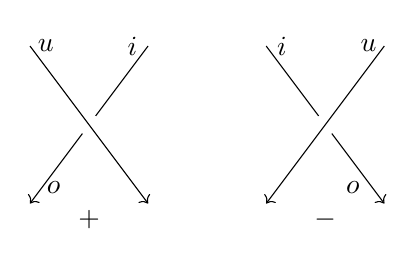
\begin{tikzpicture}
    \draw[<-] (0, -2)--(1.5, 0);
    \fill[white] (0.75, -1) circle (4pt);
    \draw[->] (0, 0)--(1.5, -2);

    \node at (0.75, -2.2) {$+$};
    \node at (0.2, 0) {$u$};
    \node at (1.3, 0) {$i$};
    \node at (0.3, -1.8) {$o$};

    \draw[->] (3, 0)--(4.5, -2);
    \fill[white] (3.75, -1) circle (4pt);
    \draw[<-] (3, -2)--(4.5, 0);
    
    \node at (3.75, -2.2) {$-$};
    \node at (3.2, 0) {$i$};
    \node at (4.3, 0) {$u$};
    \node at (4.1, -1.8) {$o$};
  \end{tikzpicture}
\end{center}
The kernel of this morphism is responsible for coloring of knot $K$. 

$a, b, c$ (and greek) are morphisms $M\to M$ (or $M\to N$ in more general case). We can assume that $c$ is a unit or even $c=1=\gamma$.

Furthermore, we can use equations above to obtain two operators $M\times M\to M\times M$ such that $(u,i)\mapsto (o, u)$ and $(i,u)\mapsto (u, o)$.

Two calculations on braids to do here, one that will give $a(a+b)=a$ and the other that states $ab=ba$ !! what is the difference when $a+b=1$ and when $a$ is not assumed to be a unit (therefore only $a^2+ab=a$)?

So now we can take a knot, its diagram and make it into a braid. A braid has a group (Burau representation, Markov knot theorem - moves) and we know that $\beta(w)v=v$ for the knot $w$ and any vector $v$.

the braid group $B_{n+1}$ with generators $\sigma_1, ..., \sigma_n$ can be send to $S_{n+1}$ with relation $\sigma\eta=\eta\sigma$ for translations that are disjoint and $\sigma\eta\sigma=\eta\sigma\eta$ ( i think ) but we might want to do something different and add a relation that sends $B_{n+1}$ to $H_{n+1}$ or however this algebra was named, using $\sigma^2+a\sigma+b=0$.

Going back to the $M\times M$ stuff -> we can have a matrix $\begin{bmatrix} 1-t & t\\ 1 & 0\end{bmatrix}$ and we can assosiate it with translation $\sigma_i$ from $B_{n+1}$ and it acts on the braid. This gives us a coloring of the braid.
}


\subsection{Coloring an unoriented knot diagram}

Let $R$ be a ring with identity and let $M$ be an $R$-module. If we consider a diagram of a knot $K$ without any orientation, the only type of crossing we will encounter is pictured in \cref{fig.1:unoriented:crossing}

\begin{figure}[h] \centering 
  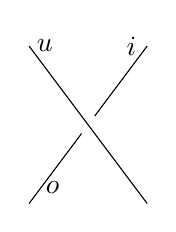
\begin{tikzpicture}
    \draw (0, -2)--(1.5, 0);
    \fill[white] (0.75, -1) circle (4pt);
    \draw (0, 0)--(1.5, -2);

    \node at (0.2, 0) {$u$};
    \node at (1.3, 0) {$i$};
    \node at (0.3, -1.8) {$o$};
  \end{tikzpicture}
  \caption{\label{fig.1:unoriented:crossing}Crossing in an unoriented knot diagram.}
\end{figure}

Notice, that rotating it by $180$ degrees changes $i$ and $o$ position (see \cref{fig.2:unoriented:crossing:floped}). Thus, segments passing under a crossing are indistinguishable. 

\begin{figure}[h] \centering 
  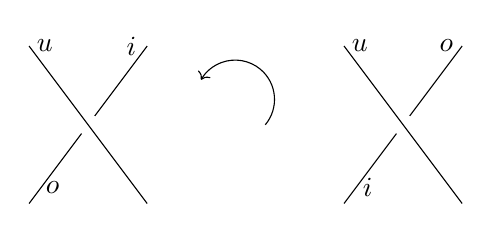
\begin{tikzpicture}
    \draw (0, -2)--(1.5, 0);
    \fill[white] (0.75, -1) circle (4pt);
    \draw (0, 0)--(1.5, -2);

    \node at (0.2, 0) {$u$};
    \node at (1.3, 0) {$i$};
    \node at (0.3, -1.8) {$o$};

    \draw[->] (3, -1) arc (-40:150:0.5);

    \draw (4, -2)--(5.5, 0);
    \fill[white] (4.75, -1) circle (4pt);
    \draw (4, 0)--(5.5, -2);

    \node at (4.2, 0) {$u$};
    \node at (5.3, 0) {$o$};
    \node at (4.3, -1.8) {$i$};
  \end{tikzpicture}
  \caption{\label{fig.2:unoriented:crossing:floped}Segments going under a crossing in an unoriented knot diagram are indistinguishable.}
\end{figure}

When $K$ has $s$ segments and $x$ crossings, we can write a labeling homomorphism
$$\phi:M^s\to M^x$$
which for segments that form a crossing pictured in \cref{fig.1:unoriented:crossing} takes value
$$\phi(u, i, o)=au+bi+co$$
for fixed $a,b,c\in\End(M)$. However, as we noted before, $i$ and $o$ are indistinguishable in \cref{fig.1:unoriented:crossing} and thus $b=c$, which yields a simpler definition:
%that assigns each element $m$ of $M^s$ an arbitrary value dependent on $a,b,c\in\End(M)$ are fixed endomorphisms and its relation to other segments. However, because $i$ and $o$ are impossible to tell apart, we must take $b=c$ and this arrive at a simpler function:
$$\phi(u,i,o)=au+b(i+o).$$

{\color{yellow}tutaj trzeba sie dokladnie zastanowic jak to idzie bardzo formalnie w zapisie
$${\color{red}\phi(u+i+o)=}au+bi+co=0$$
for $a, b, c\in \End(M)$ that are fixed for the entirety of $K$. However, because $i$ and $o$ are impossible to tell apart, we must take $b=c$ and thus arrive at a very simple equation:
%in fact have a very simple equation:
$$au+b(i+o)=0.$$
}

A coloring of a knot diagram without orientation is a labeling of its segments with elements from some module that agrees on crossings. That is, if a segment started in one crossing with label $x$ then it must be labeled with $x$ in every other crossing until another segment passes over it. Every diagram has a trivial coloring, in which every segment is labeled with the same element.

In other words, a coloring is an element from $M^s$ that agrees with $a$ and $b$ on every crossing and thus it belongs to $\ker\phi$. For $(m_1,...,m_s)\in\ker\phi$ we have a coloring such that segment $i$ is labeled with $m_i$.

{\color{yellow}If we extend the morphism $M^s\to M^x$ to an exact sequence, we obtain
$$0\to \ker\phi\to M^s\xrightarrow{\phi}M^x\to \coker\phi\to 0.$$
Module $\ker\phi$ can be viewed as a coloring of the diagram of $K$ with elements of module $M$.}

\begin{example}
  Let $M=\Z_n$, $R=\Z$, and consider the trefoil knot with $3$ segments and $3$ crossings.

  \begin{figure}[h] \centering
  \begin{tikzpicture}
    \begin{knot}[
      consider self intersections,
      flip crossing=2,
      clip width=20,
      ]
      \strand[thick]
      (90:2) to[out=180,in=-120,looseness=2]
      (-30:2) to[out=60,in=120,looseness=2]
      (210:2) to[out=-60,in=0,looseness=2] (90:2);
    \end{knot}
    \node at (130:2) {$l_1$};
    \node at (210:2.3) {$l_2$};
    \node at (-30:2.3) {$l_3$};
  \end{tikzpicture}

  \begin{tikzpicture}
  \fill (90:2.5) circle (2pt);
\fill (-30:3) circle (2pt);
\fill (210:3) circle (2pt);

\draw (90:2.5)
  \end{tikzpicture}
  \caption{An alternating diagram of trefoil knot $3_1$.}
\end{figure}

{\color{orange}TO DO: function such that $2x-y-z=0$ always when $x$ is the upper strand, using Smith's normal form show that only $\Z_3$ can be used to make a non-trivial coloring}

{\color{blue}MAYHAPSE A DIFFERENT KNOT?}

\end{example}

\subsection{The case of oriented knot diagram}



\begin{center}
  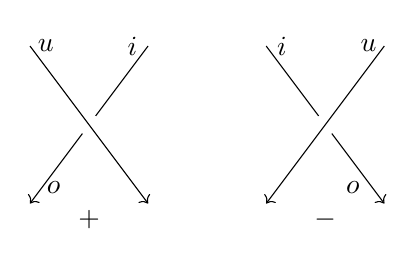
\begin{tikzpicture}
    \draw[<-] (0, -2)--(1.5, 0);
    \fill[white] (0.75, -1) circle (4pt);
    \draw[->] (0, 0)--(1.5, -2);

    \node at (0.75, -2.2) {$+$};
    \node at (0.2, 0) {$u$};
    \node at (1.3, 0) {$i$};
    \node at (0.3, -1.8) {$o$};

    \draw[->] (3, 0)--(4.5, -2);
    \fill[white] (3.75, -1) circle (4pt);
    \draw[<-] (3, -2)--(4.5, 0);
    
    \node at (3.75, -2.2) {$-$};
    \node at (3.2, 0) {$i$};
    \node at (4.3, 0) {$u$};
    \node at (4.1, -1.8) {$o$};
  \end{tikzpicture}
\end{center}





%\section{Calculating the Alexander Module}

Kinoshita-Tarasaki - does not look too promising

Conway Knot - to be examined


%\section{The case of oriented knot diagrams}

\subsection{Labeling homomorphism with orientation}

Every knot diagram has two orientations and in an oriented diagram there are two distinct types of crossings as seen in \cref{fig:3:two:types:crossings}. In such crossings segments $i$ and $o$ are easily distinguishable, allowing us to write two different elements to which labeling homomorphism $\phi$ will map segments that contribute to one crossing:
$$+:\phi(u,i,o)=au+bi+co$$
$$-:\phi(u,i,o)=\alpha u+\beta i+\gamma o.$$

\begin{figure}[h]\centering
  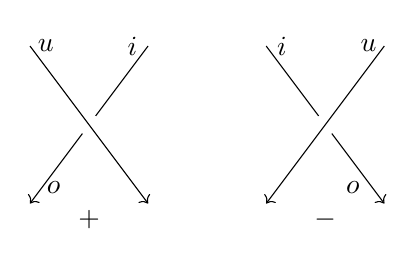
\begin{tikzpicture}
    \draw[<-] (0, -2)--(1.5, 0);
    \fill[white] (0.75, -1) circle (4pt);
    \draw[->] (0, 0)--(1.5, -2);

    \node at (0.75, -2.2) {$+$};
    \node at (0.2, 0) {$u$};
    \node at (1.3, 0) {$i$};
    \node at (0.3, -1.8) {$o$};

    \draw[->] (3, 0)--(4.5, -2);
    \fill[white] (3.75, -1) circle (4pt);
    \draw[<-] (3, -2)--(4.5, 0);
    
    \node at (3.75, -2.2) {$-$};
    \node at (3.2, 0) {$i$};
    \node at (4.3, 0) {$u$};
    \node at (4.1, -1.8) {$o$};
  \end{tikzpicture}
  \caption{\label{fig:3:two:types:crossings}Two types of crossings in oriented knot diagram.}
\end{figure}

Just as before, elements from $M^s$ that map to $0$ element in $M^x$ are responsible for coloring of diagram being examined. 


%\section{Problem}

Consider a field $\mathfrak{K}$ and the ring of polynomials with coefficients in $\mathfrak{K}$, $\mathfrak{K}[x]$. Obviously, the aforementioned ring is a principial ideal domain. We want to consider group $\Z[[M]]$, where $[M]$ is the equivalence class of all finitely generated torsion modules isomorphic to $M$ and relation $[M_2]=[M_1]+[M_3]$ defined by the existence of an exact sequence.

Any finitely generated module $M$ is isomorphic to a direct sum of cyclic modules:
$$M\cong p_1\mathfrak{K}[x]\oplus p_2\mathfrak{K}[x]\oplus...\oplus p_n\mathfrak{K}[x]$$

Moduły które mają ten sam wielomian w rozkładzie trafiają do tego samego domku.

{\color{green} If $p$, $q$ are two irreducible polynomials, then $(p)\oplus  (q)=\mathfrak{K}[x]$ (example: $x-1, x^2+1$).}


$$x^2+2x+1-(x-1)(x+3)$$


\section{Introduction}

\section{Knot coloring}

Let $R$ be any commutative ring with identity, let $M$ be a module with one generator and $\phi:M^3\to M$ be a homomorphism such that for every $m\in M$
%$M$ be any \textbf{\color{red}finitely generated} $R$-module and $\phi:M^3\to M$ be a homomorphism such that for every $m\in M$ 
\begin{equation}\label{phi allows for trivial colorings}
  \phi(m,m,m)=0.
\end{equation}
Notice that if $\phi(u,i,o)=au+bi+co$, then aforementioned equality demands that $(a+b+c)\in \ann(M)$.

Take $K$ to be any knot with diagram $D$ with $s$ arches and $x$ crossings.

\begin{lemma}
  For diagrams of knots other than $0_1$, the number of segments $s$ is equal to the number of crossings $x$.
\end{lemma}

\begin{proof}
  Every crossing has $2$ arcs that go below it and every arc has two bottom ends that are created when this segment disappears below another segment. Thus 
  $$2\cdot \#\text{arches} = \#\text{bottom ends} = 2\cdot \#\text{crossings}.$$
\end{proof}

\begin{definition}\label{coloring definition primitive}
  We say that $C\subseteq M^s$ is a \emph{coloring module} of the diagram $D$ with elements from $M$ if it 
  \begin{enumerate}
    \item {\color{orange}has $s$ generators, each corresponding to one arc of the diagram}, 
    \item and for every $u, i, o\in C$ that correspond to arcs meeting in one crossing, $\phi(u,i,o)=0$.
  \end{enumerate}
  \begin{center}
    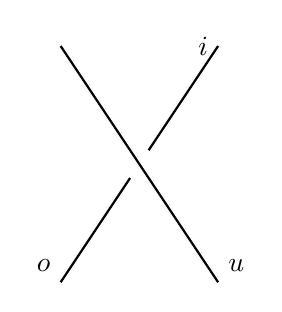
\begin{tikzpicture}
      \draw[thick] (0,0) node[above left] {$o$} --(2, 3) node [left] {$i$};
      \fill[white] (1, 1.5) circle (6pt);
      \draw[thick] (0, 3)--(2, 0) node[above right] {$u$};
    \end{tikzpicture}
  \end{center}
\end{definition}

Notice that condition stated in \cref{phi allows for trivial colorings} makes it possible to color every diagram trivially, that is by assigning the same element of $M$ to every arc.

Approach to coloring taken in \cref{coloring definition primitive} gives a lot of information about coloring with elements of one specific module and it is rather difficult to use it for other modules. Consider the following example.

\begin{example}
  Take $R=\Z$ with $\phi(x, y, z)=2x-y-z$ and consider the trefoil knot $3_1$. If we take $M=\Z$ then $K$ admits only the trivial coloring. However, if we take $M=\Z_3$ then there exists a non-trivial coloring like the one presented in \cref{trefoil knot diagram 1}.
  \begin{figure}[h]\centering
    \begin{tikzpicture}[bgnd/.style={circle, fill=white, draw=white}]
       \begin{knot}[
         consider self intersections,
         flip crossing=2,
         clip width=20,
         ]
         \strand[thick]
         (90:3) to[out=180,in=-120,looseness=2]
         (-30:3) to[out=60,in=120,looseness=2]
         (210:3) to[out=-60,in=0,looseness=2] (90:3);
       \end{knot}

       \node[bgnd] at (90:3) {$0$};
       \node[bgnd] at (-30:3) {$1$};
       \node[bgnd] at (210:3) {$2$};
  \end{tikzpicture}
 \caption{The trefoil knot $3_1$ does not allow for nontrivial coloring over $M=\Z$ but it is possible to color it with $M=\Z_3$.\label{trefoil knot diagram 1}}
\end{figure}
\end{example}

Another approach to defining coloring of a knot diagram $D$ would be by starting with identifying arches with generators $(0,..., 1, ..., 0)$ of $M^s$. Then, we might define a homomorphism
$$f:M^s\to M^x$$
such that arches building one crossing follow rules set by $\phi$.

% We might want to start defining coloring by defining a homomorphism
% $$f:M^s\to M^x$$
% which identifies coordinates with arcs in $D$ and follows $\phi$ on triples of coordinates that build one crossing. 

\begin{definition}\label{coloring definition as kernel}
  Module $\ker f$ is a coloring module of diagram $D$ with elements of $M$.
\end{definition}

\begin{corollary}
  \Cref{coloring definition primitive} and \cref{coloring definition as kernel} are equivalent for one dimensional modules.
\end{corollary}

\begin{proof}
  {\large\color{red}TO DO}
\end{proof}

Despite the fact that it is the kernel of $f$ that contains colorings, examining the matrix itself gives more information about diagram $D$. We might consider $f$ as a $s\times s$ matrix and if $R$ is a PID module, then we can represent this matrix in Smith's normal form. 
%This representation contains information about the kernel over the specific module $M$ and ring $R$ but also shows how to change $M$ and even $R$ to obtain a different coloring.

\begin{proposition}
  Let $A$ be the Smith's normal form of $f$. Columns of $A$ comprised only of zeros and zero divisors contribute to the coloring module.
\end{proposition}

\begin{proof}
  {\large\color{red}TUTAJ WOGÓLE POTRZEBA COKOLWIEK DOWODZIĆ?}
\end{proof}

%Furthermore, if $R$ is a Noetherian ring, then every finitely generated module is a quotient of a free module with the same number of generators. Thus, taking $M$ to be any finitely generated module over $R$ gives us information about coloring with any other module with equal number of generators.

If $R$ is a Noetherian ring, then every finitely generated module is a quotient of a free module with the same number of generators. Thus, we might want to take $M$ to be a finitely generated free $R$-module rather than one dimensional $R$-module. This allows us to send $M$ to any other $R$-module with at most $\dim (M)$ generators to obtain a different coloring.

Usually, it is the irreversible elements from the diagonal of Smith's form $f$ that hint at what colorings are admisible. Consider the following example.

\begin{example}
  As before, take $R=\Z$ and $\phi(x, y, z)=2x-y-z$. Taking $M=\Z$ we have $f:\Z^3\to \Z^3$ for trefoil knot to be a matrix
  $$ 
  \begin{pmatrix}
    2 & -1 & -1 \\ 
    -1 & 2 & -1 \\ 
    -1 & -1 & 2
  \end{pmatrix}
  $$ 
  with Smith's normal form
  $$
  \begin{pmatrix}
    -1 & 0 & 0 \\ 
    0 & 3 & 0\\ 
    0 & 0 & 0
  \end{pmatrix}
  $$
  Sending $M=\Z$ to $M=\Z_3$ by taking all coefficient modulo $3$ we get the new Smith's normal form of $f$ to be
  $$
  \begin{pmatrix}
    2 & 0 & 0 \\ 
    0 & 0 & 0\\ 
    0 & 0 & 0
  \end{pmatrix}
  $$
  which informs about the nontrivial coloring that was not allowed over $\Z$.
\end{example}

\section{Coloring oriented diagrams}

In the previous chapter we defined coloring of a diagram without an orientation. Such a diagram has only one type of crossing, while a diagram for which an orientation was chosen, two types of crossings are distinguishable in any knot diagram (see \cref{fig two crossings}).

\begin{figure}[h]\centering 
    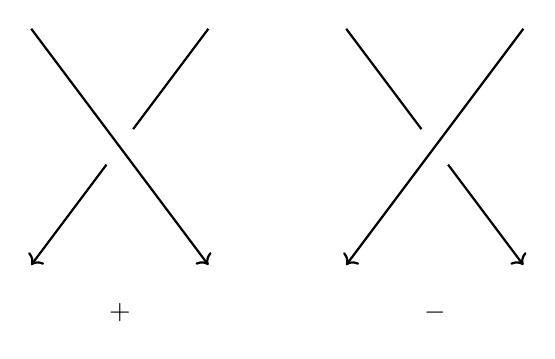
\begin{tikzpicture}
      \draw[<-, ,thick] (0,0)--(9/4, 3);
      \fill[white] (9/8, 1.5) circle (8pt);
      \draw[->, thick] (0, 3)--(9/4, 0);

      % \node at (-0.1, 0.6) {$u$};
      % \node at (9/4+0.1, 0.6) {$o$};
      % \node at (9/4+0.1, 2.4) {$i$};
      
      \draw[->, thick] (4, 3)--(4+9/4, 0);
      \fill[white] (4+9/8, 1.5) circle (8pt);
      \draw[<-, ,thick] (4,0)--(4+9/4, 3);

      % \node at (-0.1, 0.6) {$u$};
      % \node at (9/4+0.1, 0.6) {$o$};
      % \node at (9/4+0.1, 2.4) {$i$};

      \node at (9/8, -0.6) {$+$};
      \node at (4+9/8, -0.6) {$-$};
    \end{tikzpicture}
    \caption{\label{fig two crossings} Two types of crossings in oriented knot diagram.}
\end{figure}

In the case of a diagram with orientation, we must chose which type of crossing is considered by $\phi$. If not explicitly mentioned, we will choose $\phi$ to determine the rules of coloring for crossing of type $+$ in \cref{fig two crossings}. 

If $u$, $i$, $o$ are labels assigned to arches entering a $+$ type crossing that constitute a coloring, then we might write 
$$0=\phi(u, i, o)=au+bi+co.$$
Taking $c$ to be a unit, we get the following equation for the label of the arch leaving the crossing:
$$o=-c^{-1}au-c^{-1}bi.$$

Those assumption allow us to write an operator $M^2\to M^2$, which takes incoming arches as input and give segments leaving the crossing as output. The matrix of the aforementioned operator takes form
$$
A_+=\begin{pmatrix}
  -c^{-1}a & -c^{-1}b \\ 
  1 & 0
\end{pmatrix}
$$
It is convenient to take $c=-1$.

Allowing the following Reidemeister's move
\begin{center}
  \begin{tikzpicture}
    \draw[thick, ->] (1, 0) to [out=180+30, in=180-30] (1, -3);
    \fill[white] (0.5, -0.5) circle (6pt);
    \fill[white] (0.5, -2.5) circle (6pt);
    \draw[thick, ->] (0, 0) to [out=-30, in=30] (0, -3);

    \draw[dashed] (0.5, -0.5) circle (10pt);
    \draw[dashed] (0.5, -2.5) circle (10pt);
    \node at (-0.5, -0.5) {$+$};
    \node at (-0.5, -2.5) {$-$};

    \draw[thick, ->] (3, 0) to[out=-70, in=70] (3, -3);
    \draw[thick, ->] (4, 0) to[out=180+70, in=180-70] (4, -3);

    \draw[->, snake it] (1.3, -1.5)--(2.7, -1.5);
  \end{tikzpicture}
\end{center}
gives equality
$$A_-A_+=Id_2,$$
where $A_+$ is the matrix of operator for $+$ type crossing and $-$ - for the $-$ type crossing. Take 
$$
A_-=\begin{pmatrix}
  \beta & \alpha \\ 
  0 & 1 
\end{pmatrix}
$$
and consider another Reidemeister's move
\begin{center}
  \begin{tikzpicture}
    \pic[
braid/.cd,
every strand/.style={thick},
strand 1/.style={red},
strand 2/.style={green},
gap=.2,
height=1.3cm,
width=1.5cm
] {braid={s_2^{-1} s_1^{-1}  s_2^{-1} }};
\draw[thick, red, ->] (0, 0.1)--(0,0);
\draw[thick, green, ->] (1.5, 0.1)--(1.5, 0);
\draw[thick, ->] (3, 0.1)--(3, 0);

  \draw[->, snake it] (3.5, 2)--(4.5, 2);

\begin{scope}[shift={(5, 0)}]
  \pic[
    braid/.cd,
    every strand/.style={thick},
    strand 1/.style={red},
    strand 2/.style={green},
    gap=.2,
    height=1.3cm,
    width=1.5cm
  ] {braid={s_1^{-1} s_2^{-1} s_1^{-1} }};
  \draw[thick, ->] (0, 0.1)--(0,0);
  \draw[thick, ->] (1.5, 0.1)--(1.5, 0);
  \draw[thick, ->] (3, 0.1)--(3, 0);
\end{scope}
  \end{tikzpicture}
\end{center}
to obtain the following relations 
$$
\begin{cases}
  b\beta =1\\ 
  b\alpha-a=0\\
  ba = ab \\ 
  a(a+b)=a
\end{cases}
$$
We must assume that both $b$ and $\beta$ are units. In the most general situation, we have 
$$R=\Z[s, t, t^{-1}]/\{s^2+st-s\},$$
with $a$ being send to $s$ and $b$ being send to $t$. However, it can be beneficial to at first assume yet another relation: 
$$a+b=1,$$
meaning that in the ring above we have
$$s+t=1$$
and thus $R\cong \Z[t, t^{-1}]$.






















\begin{example}
  Consider knot $4_1$ with diagram $D$ as seen in \cref{fig:4_1:coloring} and ring $R=M=\Z[t, t^{-1}]$. Take function $\phi:M^3\to M$ to be defined as
  $$\phi(u, i, o)=(1-t)u+ti-o$$
  for crossing as seen in \cref{fig:crossing:4_1:example}.

  \begin{figure}[h]\centering
    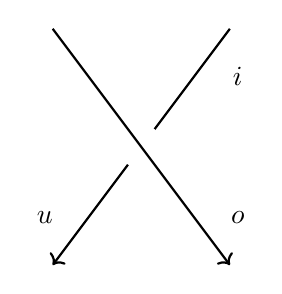
\begin{tikzpicture}
      \draw[<-, ,thick] (0,0)--(9/4, 3);
      \fill[white] (9/8, 1.5) circle (8pt);
      \draw[->, thick] (0, 3)--(9/4, 0);

      \node at (-0.1, 0.6) {$u$};
      \node at (9/4+0.1, 0.6) {$o$};
      \node at (9/4+0.1, 2.4) {$i$};
    \end{tikzpicture}
    \caption{\label{fig:crossing:4_1:example} Crossing}
  \end{figure}

  Function $f$ is then defined by matrix
  $$
  f=\begin{pmatrix}
    1-t & t & -1 & 0 \\
    t^{-1} & -1 & 0 & 1-t^{-1}\\
    0 & 1-t^{-1} & t^{-1} & -1\\
    -1 & 0 & 1-t & t
  \end{pmatrix}
  $$
  which has Smith's normal form:
  $$
  f'=\begin{pmatrix}
    -1 & 0 & 0 & 0 \\
    0 & -1 & 0 & 0\\
    0 & 0 & t^2-3t+1 & 0\\
    0 & 0 & 0 & 0\\
  \end{pmatrix}
  $$
  Notice, that $\det f'=t^2-3t+1$, which is the Alexander polynomial of $4_1$.

  \begin{figure}[h]\centering
    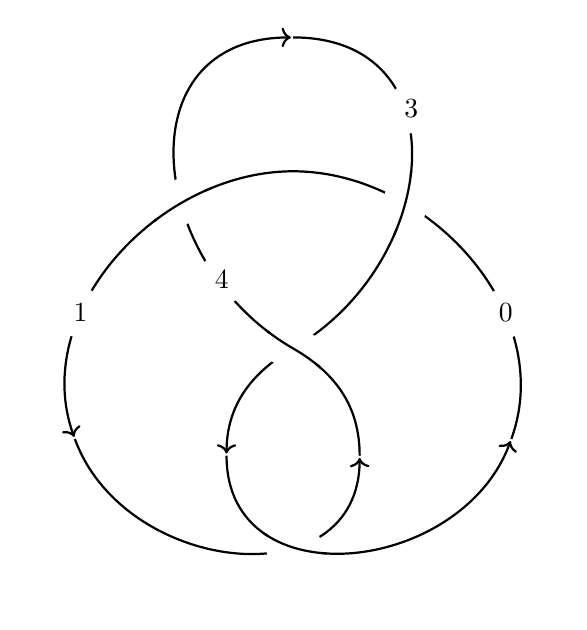
\begin{tikzpicture}[bgnd/.style={circle, fill=white, draw=white}]
      %\node[opacity=0.2] at (0,0) {\includegraphics[width=0.5\textwidth]{./rozdzialy/4_1-3d.png}};
      \coordinate (a1) at (90: 3.5);
      \coordinate (a2) at (-30:3.2);
      \coordinate (a3) at (210: 3.2);
      \coordinate (a4) at (0,-0.45);
      \coordinate (a5) at (-65:2);
      \coordinate (a6) at (180+65: 2);
      \coordinate (a7) at (90: 1.8);

      %\foreach \i in {1, ..., 7} \fill (a\i) circle (2pt);
      \begin{knot}[
        %consider self intersections,
        flip crossing=2,
        clip width=20,
        ]
        \strand[thick, ->]
        (a1) to [out=0, in=30, looseness=1.4]
        (a4) to [out=210, in=90, looseness=1] (a6);
        \strand[thick, ->]
        (a6) to [out=-90, in=250, looseness=1.3] (a2);
        \strand[thick, ->] (a2) to[out=70, in=0] (a7) to[out=180, in=110] (a3);
        \strand[thick, ->] (a3) to[out=290, in=-90, looseness=1.3] (a5);
        \strand[thick, ->] (a5) to[out=90, in=-30, looseness=1] (a4) to [out=150, in=180, looseness=1.4] (a1);
      \end{knot}

      \node[bgnd] at (60:3) {$3$};
      \node[bgnd] at (0:2.7) {$0$};
      \node[bgnd] at (-180:2.7) {$1$};
      \node[bgnd] at (155:1) {$4$};
    \end{tikzpicture}
    \caption{\label{fig:4_1:coloring} Coloring of knot $4_1$ with elements from $\Z_5$.}
  \end{figure}

  Now, consider a homomorphism $\Z[t, t^{-1}]\to \Z$ that sends $t\mapsto -1$. This yields a new matrix for $f$, with Smith's normal form:
  $$f=\begin{pmatrix}
    -1 & 0 & 0 & 0\\
    0 & 1 & 0 & 0\\
    0 & 0 & 5 & 0\\
    0 & 0 & 0 & 0
  \end{pmatrix}$$
  Now, the $\coker f=\Z\oplus \Z_5$ which hints at existence of coloring using elements from $\Z_5$. One of those colorings is presented in \cref{fig:4_1:coloring}.


%  Take $K=4_1$ and $R=\Z$, which takes $t=1$ and $s=2$. At the beginning, $M=\Z$.
%
%  \begin{center}
%    \begin{tikzpicture}
%      %\node[opacity=0.2] at (0,0) {\includegraphics[width=0.5\textwidth]{./rozdzialy/4_1-3d.png}};
%      \coordinate (a1) at (90: 3.5);
%      \coordinate (a2) at (-30:3.2);
%      \coordinate (a3) at (210: 3.2);
%      \coordinate (a4) at (0,-0.45);
%      \coordinate (a5) at (-65:2);
%      \coordinate (a6) at (180+65: 2);
%      \coordinate (a7) at (90: 1.8);
%
%      %\foreach \i in {1, ..., 7} \fill (a\i) circle (2pt);
%      \begin{knot}[
%        %consider self intersections,
%        flip crossing=2,
%        clip width=20,
%        ]
%        \strand[thick, ->]
%        (a1) to [out=0, in=30, looseness=1.4]
%        (a4) to [out=210, in=90, looseness=1] (a6);
%        \strand[thick, ->]
%        (a6) to [out=-90, in=250, looseness=1.3] (a2);
%        \strand[thick, ->] (a2) to[out=70, in=0] (a7) to[out=180, in=110] (a3);
%        \strand[thick, ->] (a3) to[out=290, in=-90, looseness=1.3] (a5);
%        \strand[thick, ->] (a5) to[out=90, in=-30, looseness=1] (a4) to [out=150, in=180, looseness=1.4] (a1);
%      \end{knot}
%      \node at (60:3.5) {$A$};
%      \node at (-30:3.6) {$B$};
%      \node at (160:2.7) {$C$};
%      \node at (1.1, -1.3) {$D$};
%
%      \draw[dashed] (a4) circle (0.4);
%      \node at (-0.8, -0.5) {$2$};
%
%      \draw[dashed] (45:2) circle (0.4);
%      \node at (35: 2.6) {$1$};
%
%      \draw[dashed] (0, -2.9) circle (0.4);
%      \node at (0, -3.6) {$3$};
%
%      \draw[dashed] (135:2) circle (0.4);
%      \node at (145:2.6) {$4$};
%    \end{tikzpicture}
%  \end{center}
%  $$f=\begin{pmatrix}
%    2 & -1 & -1 & 0\\
%    -1 & -1 & 0 & 2\\
%    0 & 2 & -1 & -1 \\
%    -1 & 0 & 2 & -1
%    \end{pmatrix}$$
%    in normal form:
%  $$\begin{pmatrix}
%    -1 & 0 & 0 & 0\\
%    0 & 1 & 0 & 0\\
%    0 & 0 & 5 & 0\\
%    0 & 0 & 0 & 0
%  \end{pmatrix}$$
%  Now we know that $\ker f=\Z$ and $\coker f=\Z_5\oplus \Z$. Thus there is only a trivial coloring over $\Z$ but if we change $\Z$ to $\Z_5$ we get
%  $$\begin{pmatrix}
%    -1 & 0 & 0 & 0\\
%    0 & 1 & 0 & 0\\
%    0 & 0 & 0 & 0\\
%    0 & 0 & 0 & 0
%  \end{pmatrix}$$
%  and now $\ker f'=\Z_5\oplus \Z_5$ and $\coker = \Z_5\oplus\Z_5$. Thus there is a coloring using elements of $\Z_5$, for example:
%
%  In a more general case, we would orient the diagram and use $\Z[\Z]=\Z[t, t^{-1}]$ as the ring:
%  $$
%  f=\begin{pmatrix}
%    1-t & t & -1 & 0 \\
%    t^{-1} & -1 & 0 & 1-t^{-1}\\
%    0 & 1-t^{-1} & t^{-1} & -1\\
%    -1 & 0 & 1-t & t
%  \end{pmatrix}
%  $$
%  $$
%  \begin{pmatrix}
%    -1 & 0 & 0 & 0 \\
%    0 & -1 & 0 & 0\\
%    0 & 0 & t^2-3t+1 & 0\\
%    0 & 0 & 0 & 0\\
%  \end{pmatrix}
%  $$
%  and the Alexander polynomial of $4_1$ is equal to $t-3+t^{-1}$, which is the same up to multiplication by a unit to the last term of the Smith's normal form.
\end{example}










% \bigskip
%
% \rule{\textwidth}{1pt}
% \bigskip
%
% In order for trivial coloring to work, $\phi(m,m,m)=0$ for all $m\in M$. This means that if we take $\phi(u, v, w)=au+bv+cw$ then $(a+b+c)\in\ann(M)$.
%
% In the most general case, $R=\Z[s, t, t^{-1}]/\{s(s+t-1)\}$ and $\phi(u,v,w)=su+tv-w$.
%
% Given those we can define $f:M^s\to M^x$, which assigns values from $M$ to segments of $D$ according to the rules set by $\phi$.
%
% This yields an exact sequence
% \begin{center}\begin{tikzcd}
%   0\arrow[r] & \ker f\arrow[r, hookrightarrow] & M^s\arrow[r, "f"] & M^x \arrow[r, two heads] & \coker f \arrow[r] & 0 
% \end{tikzcd}\end{center}
%
% We know that $\ker f$ always contains colorings - especially the trivial one. We expect $\coker f$ to contain some information about non-trivial colorings admissible.
%
% \subsection{Smith's normal form \textquestiondown and connection to Alexander polynomial?}
%
% Function $f$ can be expressed as a $s\times x$ matrix with elements from $M$ - we can make it into "diagonal form" where non-zero elements lower are divisible by elements at the top. This gives us information about $\ker f$ and $\coker f$.
%
% \begin{example}
%   Consider knot $4_1$ with diagram $D$ as seen in \cref{fig:4_1:coloring} and ring $R=M=\Z[t, t^{-1}]$. Take function $\phi:M^3\to M$ to be defined as 
%   $$\phi(u, i, o)=(1-t)u+ti-o$$
%   for crossing as seen in \cref{fig:crossing:4_1:example}.
%
%   \begin{figure}[h]\centering
%     \begin{tikzpicture}
%       \draw[<-, ,thick] (0,0)--(9/4, 3);
%       \fill[white] (9/8, 1.5) circle (8pt); 
%       \draw[->, thick] (0, 3)--(9/4, 0);
%
%       \node at (-0.1, 0.6) {$u$};
%       \node at (9/4+0.1, 0.6) {$o$};
%       \node at (9/4+0.1, 2.4) {$i$};
%     \end{tikzpicture}
%     \caption{\label{fig:crossing:4_1:example} Crossing}
%   \end{figure}
%
%   Function $f$ is then defined by matrix
%   $$
%   f=\begin{pmatrix}
%     1-t & t & -1 & 0 \\ 
%     t^{-1} & -1 & 0 & 1-t^{-1}\\ 
%     0 & 1-t^{-1} & t^{-1} & -1\\ 
%     -1 & 0 & 1-t & t
%   \end{pmatrix}
%   $$
%   which has Smith's normal form:
%   $$
%   f'=\begin{pmatrix}
%     -1 & 0 & 0 & 0 \\
%     0 & -1 & 0 & 0\\ 
%     0 & 0 & t^2-3t+1 & 0\\ 
%     0 & 0 & 0 & 0\\ 
%   \end{pmatrix}
%   $$
%   Notice, that $\det f'=t^2-3t+1$, which is the Alexander polynomial of $4_1$.
%
%   \begin{figure}[h]\centering
%     \begin{tikzpicture}[bgnd/.style={circle, fill=white, draw=white}]
%       %\node[opacity=0.2] at (0,0) {\includegraphics[width=0.5\textwidth]{./rozdzialy/4_1-3d.png}};
%       \coordinate (a1) at (90: 3.5);
%       \coordinate (a2) at (-30:3.2);
%       \coordinate (a3) at (210: 3.2);
%       \coordinate (a4) at (0,-0.45);
%       \coordinate (a5) at (-65:2);
%       \coordinate (a6) at (180+65: 2);
%       \coordinate (a7) at (90: 1.8);
%
%       %\foreach \i in {1, ..., 7} \fill (a\i) circle (2pt);
%       \begin{knot}[
%         %consider self intersections,
%         flip crossing=2,
%         clip width=20,
%         ]
%         \strand[thick, ->]
%         (a1) to [out=0, in=30, looseness=1.4] 
%         (a4) to [out=210, in=90, looseness=1] (a6);
%         \strand[thick, ->]
%         (a6) to [out=-90, in=250, looseness=1.3] (a2);
%         \strand[thick, ->] (a2) to[out=70, in=0] (a7) to[out=180, in=110] (a3);
%         \strand[thick, ->] (a3) to[out=290, in=-90, looseness=1.3] (a5);
%         \strand[thick, ->] (a5) to[out=90, in=-30, looseness=1] (a4) to [out=150, in=180, looseness=1.4] (a1);
%       \end{knot}
%
%       \node[bgnd] at (60:3) {$3$};
%       \node[bgnd] at (0:2.7) {$0$};
%       \node[bgnd] at (-180:2.7) {$1$};
%       \node[bgnd] at (155:1) {$4$};
%     \end{tikzpicture}
%     \caption{\label{fig:4_1:coloring} Coloring of knot $4_1$ with elements from $\Z_5$.}
%   \end{figure}
%
%   Now, consider a homomorphism $\Z[t, t^{-1}]\to \Z$ that sends $t\mapsto -1$. This yields a new matrix for $f$, with Smith's normal form:
%   $$f=\begin{pmatrix}
%     -1 & 0 & 0 & 0\\ 
%     0 & 1 & 0 & 0\\
%     0 & 0 & 5 & 0\\ 
%     0 & 0 & 0 & 0
%   \end{pmatrix}$$
%   Now, the $\coker f=\Z\oplus \Z_5$ which hints at existence of coloring using elements from $\Z_5$. One of those colorings is presented in \cref{fig:4_1:coloring}.
%
%
% %  Take $K=4_1$ and $R=\Z$, which takes $t=1$ and $s=2$. At the beginning, $M=\Z$.
% %
% %  \begin{center}
% %    \begin{tikzpicture}
% %      %\node[opacity=0.2] at (0,0) {\includegraphics[width=0.5\textwidth]{./rozdzialy/4_1-3d.png}};
% %      \coordinate (a1) at (90: 3.5);
% %      \coordinate (a2) at (-30:3.2);
% %      \coordinate (a3) at (210: 3.2);
% %      \coordinate (a4) at (0,-0.45);
% %      \coordinate (a5) at (-65:2);
% %      \coordinate (a6) at (180+65: 2);
% %      \coordinate (a7) at (90: 1.8);
% %
% %      %\foreach \i in {1, ..., 7} \fill (a\i) circle (2pt);
% %      \begin{knot}[
% %        %consider self intersections,
% %        flip crossing=2,
% %        clip width=20,
% %        ]
% %        \strand[thick, ->]
% %        (a1) to [out=0, in=30, looseness=1.4] 
% %        (a4) to [out=210, in=90, looseness=1] (a6);
% %        \strand[thick, ->]
% %        (a6) to [out=-90, in=250, looseness=1.3] (a2);
% %        \strand[thick, ->] (a2) to[out=70, in=0] (a7) to[out=180, in=110] (a3);
% %        \strand[thick, ->] (a3) to[out=290, in=-90, looseness=1.3] (a5);
% %        \strand[thick, ->] (a5) to[out=90, in=-30, looseness=1] (a4) to [out=150, in=180, looseness=1.4] (a1);
% %      \end{knot}
% %      \node at (60:3.5) {$A$};
% %      \node at (-30:3.6) {$B$};
% %      \node at (160:2.7) {$C$};
% %      \node at (1.1, -1.3) {$D$};
% %
% %      \draw[dashed] (a4) circle (0.4);
% %      \node at (-0.8, -0.5) {$2$};
% %
% %      \draw[dashed] (45:2) circle (0.4);
% %      \node at (35: 2.6) {$1$};
% %
% %      \draw[dashed] (0, -2.9) circle (0.4);
% %      \node at (0, -3.6) {$3$};
% %
% %      \draw[dashed] (135:2) circle (0.4);
% %      \node at (145:2.6) {$4$};
% %    \end{tikzpicture}
% %  \end{center}
% %  $$f=\begin{pmatrix} 
% %    2 & -1 & -1 & 0\\ 
% %    -1 & -1 & 0 & 2\\ 
% %    0 & 2 & -1 & -1 \\ 
% %    -1 & 0 & 2 & -1
% %    \end{pmatrix}$$
% %    in normal form:
% %  $$\begin{pmatrix}
% %    -1 & 0 & 0 & 0\\ 
% %    0 & 1 & 0 & 0\\
% %    0 & 0 & 5 & 0\\ 
% %    0 & 0 & 0 & 0
% %  \end{pmatrix}$$
% %  Now we know that $\ker f=\Z$ and $\coker f=\Z_5\oplus \Z$. Thus there is only a trivial coloring over $\Z$ but if we change $\Z$ to $\Z_5$ we get 
% %  $$\begin{pmatrix}
% %    -1 & 0 & 0 & 0\\ 
% %    0 & 1 & 0 & 0\\
% %    0 & 0 & 0 & 0\\ 
% %    0 & 0 & 0 & 0
% %  \end{pmatrix}$$
% %  and now $\ker f'=\Z_5\oplus \Z_5$ and $\coker = \Z_5\oplus\Z_5$. Thus there is a coloring using elements of $\Z_5$, for example:
% %
% %  In a more general case, we would orient the diagram and use $\Z[\Z]=\Z[t, t^{-1}]$ as the ring:
% %  $$
% %  f=\begin{pmatrix}
% %    1-t & t & -1 & 0 \\ 
% %    t^{-1} & -1 & 0 & 1-t^{-1}\\ 
% %    0 & 1-t^{-1} & t^{-1} & -1\\ 
% %    -1 & 0 & 1-t & t
% %  \end{pmatrix}
% %  $$
% %  $$
% %  \begin{pmatrix}
% %    -1 & 0 & 0 & 0 \\
% %    0 & -1 & 0 & 0\\ 
% %    0 & 0 & t^2-3t+1 & 0\\ 
% %    0 & 0 & 0 & 0\\ 
% %  \end{pmatrix}
% %  $$
% %  and the Alexander polynomial of $4_1$ is equal to $t-3+t^{-1}$, which is the same up to multiplication by a unit to the last term of the Smith's normal form.
% \end{example}
%
%
%
%
%
%
%
%
%
%
%
%
%
%
% %{\color{blue}
% %Let $D$ be a diagram of knot $K$ with $s$ segments and $x$ crossings.  We will take $R$ to be a commutative ring with identity and $M$ to be any $R$-module. Looking at each crossing locally, we see that exactly $3$ segments will meet and thus we need a function 
% %$$\phi:M^3\to M$$ 
% %which assigns value to a crossing based on the values inscribed on segments from which it is constructed.  
% %
% %We can now extend the function $\phi$ to work on the whole diagram $D$, which yields a new function 
% %$$f:M^s\to M^x,$$
% %that assigns values from $M$ to line segments from $D$. We say that $(x_1,...,x_s)\in M^s$ is a \emph{coloring of $D$} if 
% %$$(x_1,...,x_s)\in\ker f,$$
% %or in other words: $f(x_1,...,x_s)=0$.
% %
% %We want any trivial coloring to always be admissible and thus $a$, $b$, $c$ in the definition of $\phi$ must be from $\ann(M)$:
% %$$0=\phi(m,m,m)=am+bm+cm=(a+b+c)m$$
% %for all $m\in M$.
% %
% %On the other hand, function $\phi$ can be used to construct an operator $M^2\to M^2$ which takes segments entering a crossing and returns segments leaving it. In the case of a diagram with defined orientation, we can distinguish two types of crossings (look at \cref{fig:1:two:types:crossings}) and so $\phi$ will actually give rise to two different operators $A_{\pm}:M^2\to M^2$, whose composition is identity on $M^2$ (this is a direct result of Reidemeister moves).
% %
% %\begin{figure}[h]\centering
% %  \begin{tikzpicture}
% %    \draw[<-, thick] (0, -2)--(1.5, 0);
% %    \fill[white] (0.75, -1) circle (6pt);
% %    \draw[->, thick] (0, 0)--(1.5, -2);
% %
% %    \node at (0.75, -2.2) {$+$};
% %    %\node at (0.2, 0) {$u$};
% %    %\node at (1.3, 0) {$i$};
% %    %\node at (0.3, -1.8) {$o$};
% %
% %    \draw[->, thick] (3, 0)--(4.5, -2);
% %    \fill[white] (3.75, -1) circle (6pt);
% %    \draw[<-, thick] (3, -2)--(4.5, 0);
% %    
% %    \node at (3.75, -2.2) {$-$};
% %    %\node at (3.2, 0) {$i$};
% %    %\node at (4.3, 0) {$u$};
% %    %\node at (4.1, -1.8) {$o$};
% %  \end{tikzpicture}
% %  \caption{\label{fig:1:two:types:crossings}Two types of crossings in oriented knot diagram.}
% %\end{figure}
% %
% %{\color{red}
% %Having constructed two $2\times 2$ matrices, $A_+$ and $A_-$, from $\phi$ we can now represent $D$ as an element of braid group $W\in B_n$. This group has $(n-1)$ generators, $\sigma_1,...,\sigma_{n-1}$, to which we can assign matrices 
% %$$\sigma_i=\left[
% %\begin{array}{c|c|c}
% %  Id_{i-1} & 0 & 0 \\ 
% %  \hline 
% %  0 & A_+  & 0 \\ 
% %  \hline 
% %  0 & 0 & Id_{n-i-1}
% %\end{array}\right]
% %$$
% %Using these matrices we can now color this braid representation of $D$ to obtain a smaller matrix $B(W)$ than the one describing $f$ above. We will say that $(m_1,...,m_{s'})$ is a coloring of this braid diagram $W$ (which can have $s'\neq s$ segments) if $(m_1,...,m_{s'})\in\ker B(W)$.
% %}
% %}
% %


\subsection{Misc}

\begin{center}
  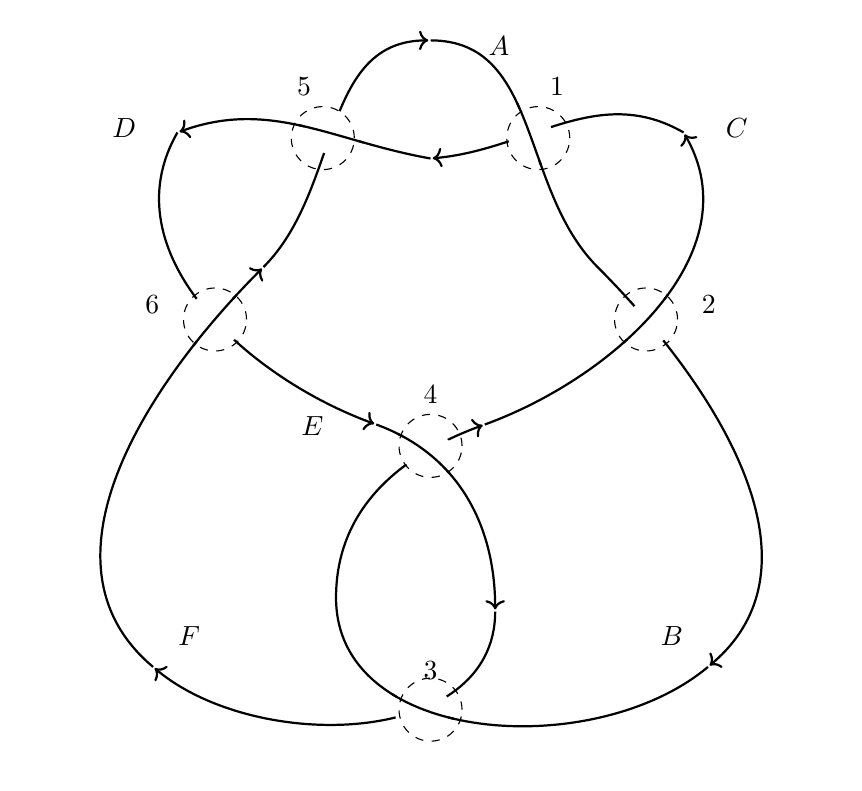
\begin{tikzpicture}[bgnd/.style={circle, fill=white, draw=white}]
    %\node[opacity=0.2] at (0,0) {\includegraphics[width=0.7\textwidth]{./rozdzialy/6_1-3d.png}};

    \coordinate (a0) at (0,0);
    \coordinate (a1) at (90:5);
    \coordinate (a2) at (45:3);
    \coordinate (a3) at (-40:4.6);
    \coordinate (a4) at (-120:2.4);
    \coordinate (a5) at (10:0.7);
    \coordinate (a6) at (50:5);
    \coordinate (a7) at (90:3.5);
    \coordinate (a8) at (180-50:5);
    \coordinate (a9) at (170:0.7);
    \coordinate (a10) at (-70:2.4);
    \coordinate (a11) at (220:4.6);
    \coordinate (a12) at (180-45:3);

    %\foreach \i in {0,...,12} \fill (a\i) circle (2pt);

    \begin{knot}[
      clip width=20, 
      flip crossing=1,
      flip crossing=3,
      flip crossing=6
      ]
      \strand[thick, ->] (a1) to[out=0, in=90+45] (a2) to[out=-45, in=40] (a3);
      \strand[thick, ->] (a3) to[out=220, in=-90] (a4) to[out=90, in=200] (a5);
      \strand[thick, ->] (a5) to[out=20, in=-60] (a6);
      \strand[thick, ->] (a6) to[out=150, in=5] (a7);
      \strand[thick, ->] (a7) to[out=170, in=20] (a8);
      \strand[thick, ->] (a8) to[out=240, in=160] (a9);
      \strand[thick, ->] (a9) to[out=-20, in=90] (a10);
      \strand[thick, ->] (a10) to[out=-90, in=-40] (a11);
      \strand[thick, ->] (a11) to[out=140, in=180+45] (a12);
      \strand[thick, ->] (a12) to[out=45, in=180] (a1);
    \end{knot}

    \node at (80: 5) {$A$};
    \node at (-40:4) {$B$};
    \node at (45:5.5) {$C$};
    \node at (135:5.5) {$D$};
    \node at (-1.5,0.1) {$E$};
    \node at (220:4) {$F$};
    
    \node[bgnd] at (70:4.7) {$1$};
    \node[bgnd] at (25:3.9) {$2$};
    \node[bgnd] at (-90:3) {$3$};
    \node[bgnd] at (90:0.5) {$4$};
    \node[bgnd] at (110:4.7) {$5$};
    \node[bgnd] at (180-25:3.9) {$6$};

    \draw[dashed] (70: 4) circle (0.4);
    \draw[dashed] (28: 3.1) circle (0.4);
    \draw[dashed] (-90:3.5) circle (0.4);
    \draw[dashed] (-90:0.15) circle (0.4);
    \draw[dashed] (180-28:3.1) circle (0.4);
    \draw[dashed] (110:4) circle (0.4);
  \end{tikzpicture}
\end{center}
Tutaj mamy
$$f=\begin{pmatrix}
  -1 & 0 & 0 & 0 & 0 & 0 \\ 
  0 & -1 & 0 & 0 & 0 & 0 \\ 
  0 & 0 & t & 0 & 0 & 0 \\ 
  0 & 0 & 0 & t & 0 & 0 \\ 
  0 & 0 & 0 & 0 & -2x^{-2}+5x^{-1}-2 & 0 \\ 
  0 & 0 & 0 & 0 & 0 & 0 
\end{pmatrix}$$


\bibliographystyle{plain}
\bibliography{literatura}
 
\end{document}
